\chapter{Planificación del proyecto}\label{chap:planif}
La planificación de un proyecto es fundamental para su correcto funcionamiento y desarrollo,
dentro de los plazos y costes establecidos. Se presenta un primer apartado de metodología, un
segundo apartado con la planificación inicial para posteriormente inferir en base a esta el
presupuesto inicial


\section{Metodología}\label{sec:metodología}
En este capítulo se aborda la metodología adoptada para el desarrollo del proyecto, fundamentada
en principios ágiles y enfocada en la entrega continua de valor. La elección de \textit{Scrum},
una metodología que permite elaborar productos software de manera incremental, revisando el
producto continuamente y adaptándolo a las necesidades del cliente, como marco de trabajo subraya
nuestro compromiso con la adaptabilidad y la mejora continua del producto.

La estructura de este capítulo se organiza en torno a la descripción detallada de la metodología
\textit{Scrum}, la visualización de la planificación y las estrategias de comunicación adoptadas.
A través de esta metodología, buscamos optimizar los recursos disponibles, ajustarnos a los plazos
establecidos y garantizar la calidad del producto final.

La implementación de \textit{Scrum} se complementa con herramientas de visualización y gestión de
proyectos, como los tableros \textit{Kanban}, que facilitan la organización y seguimiento de
las tareas. Además, se pone especial énfasis en la comunicación efectiva dentro del equipo de
desarrollo y con los stakeholders, asegurando así una alineación constante con los objetivos del
proyecto. Existen otras variantes de los tableros \textit{Kanban} que se pueden utilizar para
visualizar el progreso de las tareas, pero en este proyecto se ha elegido esta alternativa para
facilitar la visualización de las tareas y su estado.

Este enfoque metodológico no solo refleja la planificación y ejecución del proyecto, sino que
también establece las bases para una gestión eficaz, adaptativa y orientada a resultados.

\newpage{}
\subsection{Scrum}\label{subsec:scrum}
Para la planificación del proyecto se ha escogido \textit{Scrum}, una metodología ``ágil'' que se
basa en la realización de iteraciones cortas y en la adaptación a los cambios. La metodología
\textit{Scrum} se estructura en \textit{sprints} (iteraciones cortas de una duración fija),
en las que se llevan a cabo una serie de tareas que se han planificado previamente.

El primer paso de la metodología \textit{Scrum} es la creación de un \textit{product backlog},
una lista ordenada de las tareas a realizar durante el desarrollo del producto, a partir de los
requisitos del sistema, que a su vez son una versión refinada de los requisitos iniciales del
proyecto. A partir de este \textit{product backlog} se planifican las tareas que se llevarán
a cabo en cada \textit{sprint}, de manera que sea posible cumplir con los objetivos del proyecto
en el tiempo establecido.

A diferencia de metodologías tradicionales o \emph{en cascada}, \textit{Scrum} permite la adaptación
a los cambios y la mejora continua del producto, ya que se revisa y se adapta en cada \textit{sprint}
según las necesidades del cliente y del equipo de desarrollo. Por otro lado, \textit{Scrum} se
diferencia de otras metodologías ágiles como \textit{XP} en que no se centra tanto en las
prácticas de desarrollo, sino en la gestión del proyecto y en la entrega de valor al cliente.

\begin{minipage}{\linewidth}
	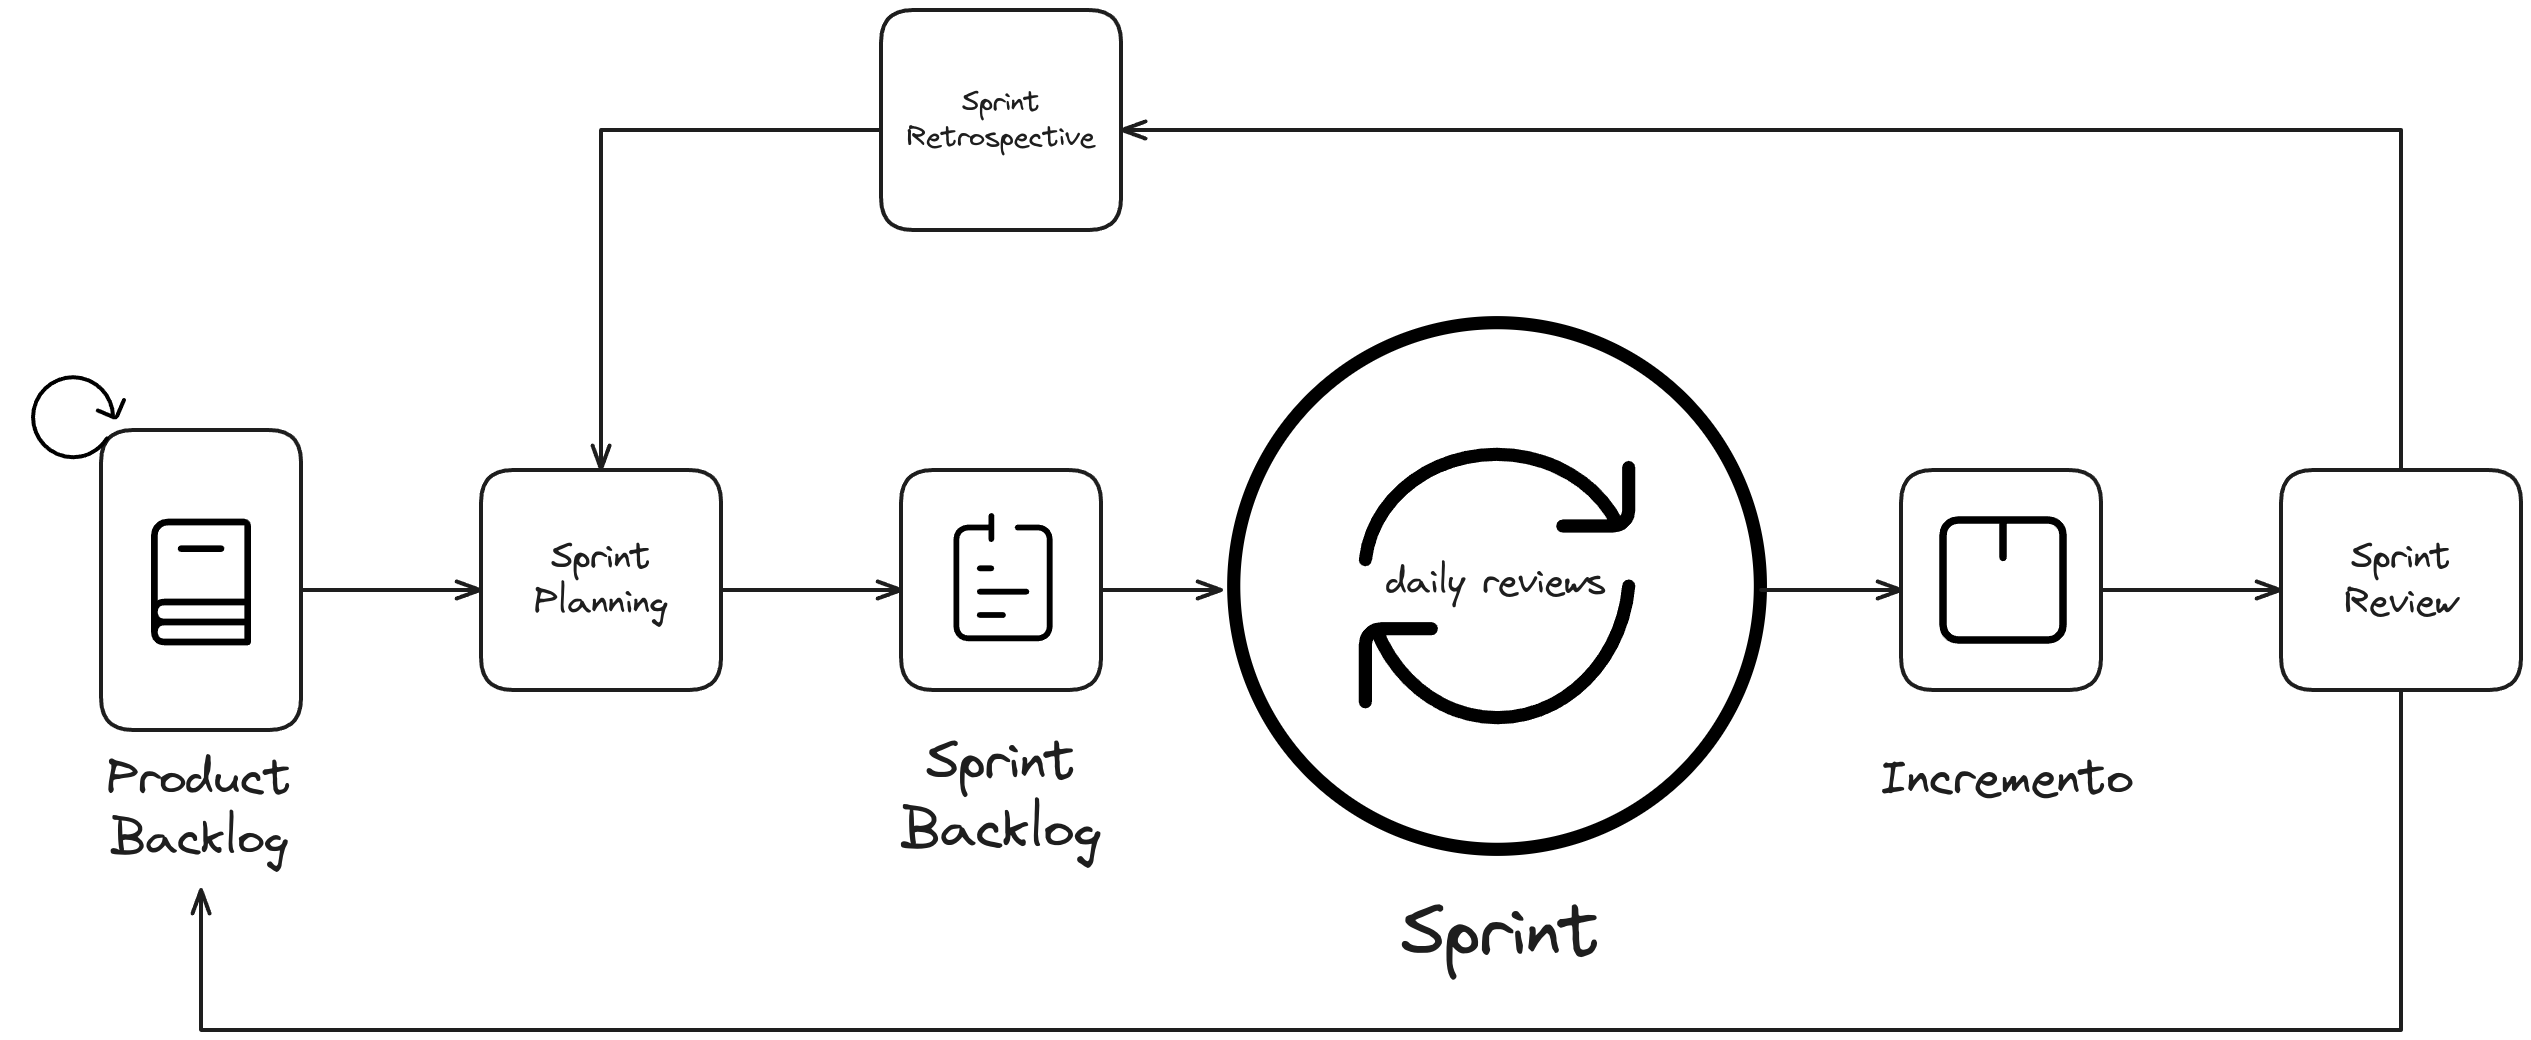
\includegraphics[width=0.85\textwidth]{scrum.png}
	\captionof{figure}{Diagrama de la metodología \textit{Scrum}}
\end{minipage}

\paragraph{Roles}
En \textit{Scrum} se distinguen tres roles principales:

\begin{itemize}
	\item \textbf{Product Owner}: es la persona responsable de definir los requisitos del producto
		y de priorizar las tareas del \textit{product backlog}. Es el enlace entre el equipo de
		desarrollo y el cliente, y es el responsable de garantizar que el producto cumple con las
		expectativas del cliente. En el caso de este proyecto, el \textit{Product Owner} es el
		director tecnológico de la empresa.
	\item \textbf{Scrum Master}: es la persona responsable de garantizar que el equipo de desarrollo
		sigue la metodología \textit{Scrum} y de eliminar los obstáculos que puedan surgir durante
		el desarrollo del proyecto. El \textit{Scrum Master} es el encargado de organizar las
		reuniones diarias y de asegurar que el equipo de desarrollo cumple con los plazos y los
		objetivos del proyecto. En este proyecto, el \textit{Scrum Master} son los tutores académicos
		del proyecto.
	\item \textbf{Equipo de desarrollo}: es el equipo encargado de llevar a cabo las tareas del
		\textit{product backlog} y de entregar el producto final. El equipo de desarrollo es
		autoorganizado y multidisciplinario, y se organiza en torno a las tareas que se van a
		realizar en cada \textit{sprint}. Para este proyecto, el ``equipo'' de desarrollo está
		constituido únicamente por el alumno, que se encarga de todas las tareas de desarrollo y
		documentación.
	\item \textbf{Stakeholders}: son las partes interesadas en el proyecto, como los clientes,
		los usuarios finales y los patrocinadores, que desconocen el proceso de desarrollo pero
		tienen un interés en el producto final y en su correcto funcionamiento.
\end{itemize}

\subsection{Visualización de la planificación}\label{subsec:visual_planif}
Para la visualización de la planificación se ha utilizado la herramienta de gestión de proyectos
de \textit{GitHub}, que permite múltiples visualizaciones de tareas e \textit{issues} en tableros
separados.

\begin{itemize}
	\item Se utiliza un tablero de \textit{requisitos} al estilo \textit{Kanban} para visualizar
		los requisitos del proyecto y su estado, siguiendo con la metodología \textit{Scrum}.
		Un tablero \textit{Kanban} es una herramienta visual que permite gestionar el flujo de
		de trabajo de un proyecto por ``sprints'', dividiendo las tareas en columnas y moviéndolas
		de una columna a otra según su estado.

		\begin{figure}[H]
			\centering
			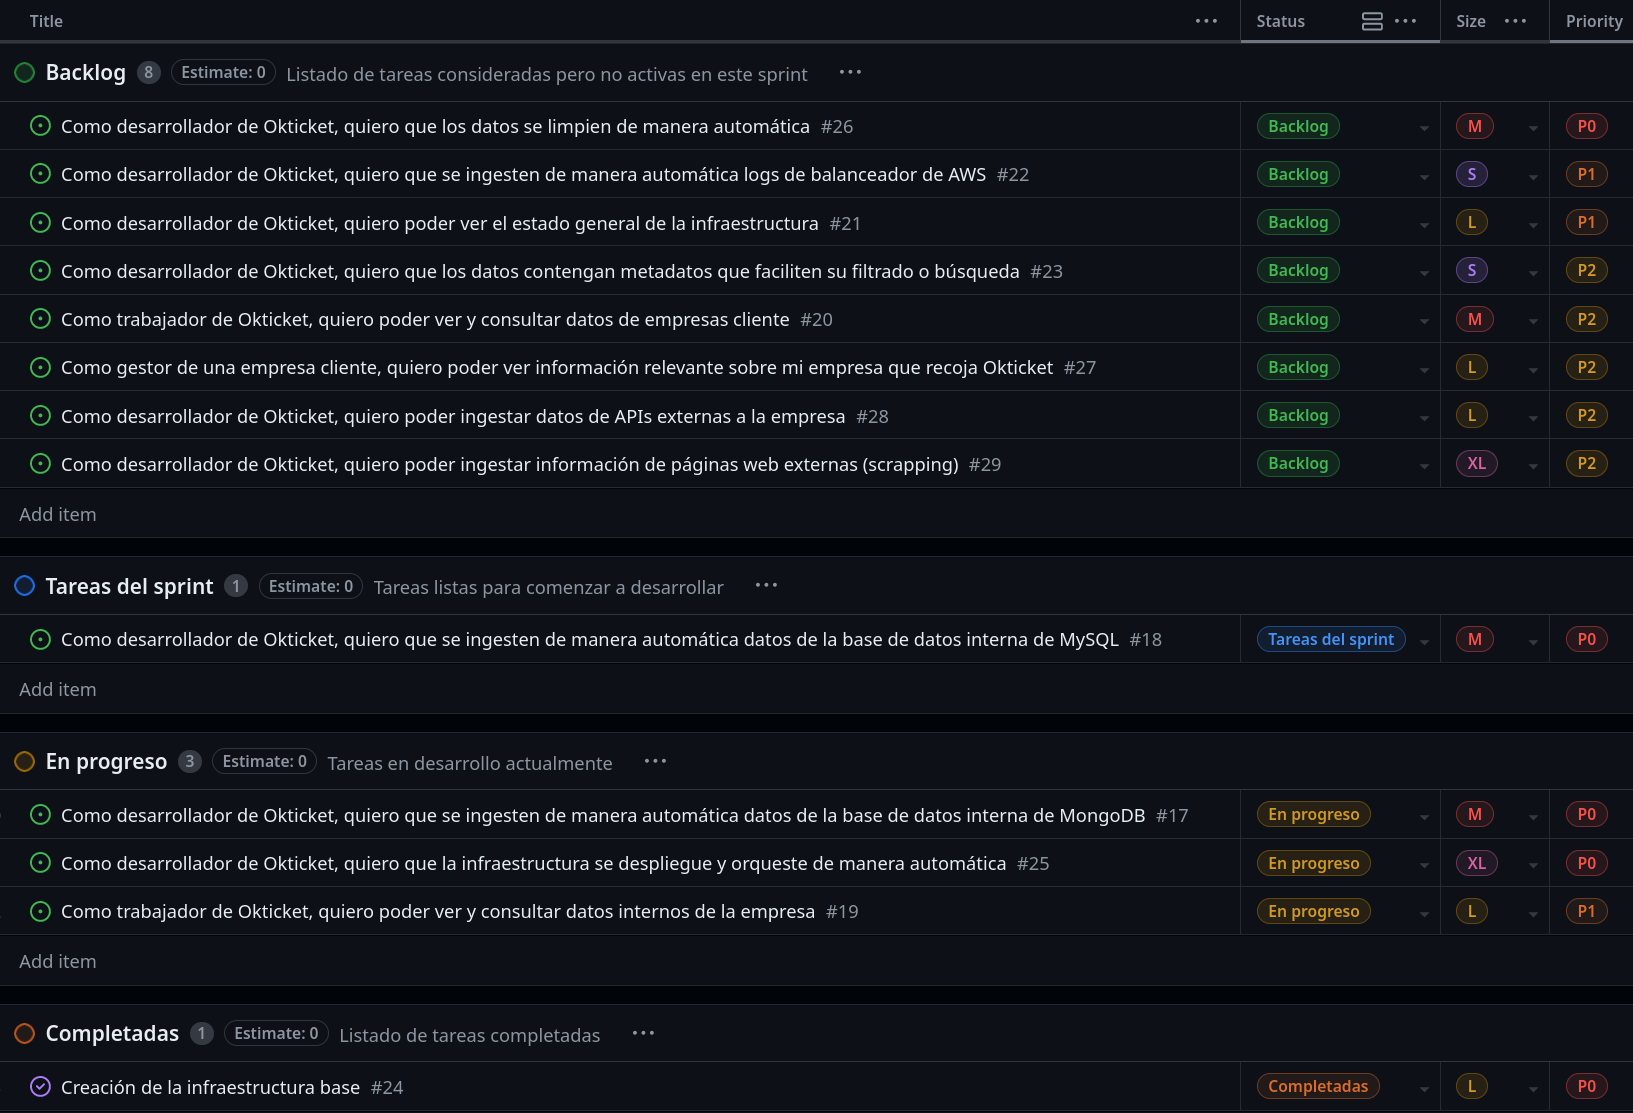
\includegraphics[width=\textwidth]{kanban.png}
			\caption{Tablero \textit{Kanban} del proyecto}
			\label{fig:kanban}
		\end{figure}
	\item Se utiliza un \textit{roadmap} de apartados de la memoria, separado del tablero de desarrollo
		normal, donde se visualiza su estado y sus fechas límite. Este \textit{roadmap} no está
		relacionado con la metodología \textit{Scrum}, sino que se ha creado a propósito para facilitar
		la visualización del progreso de cada sección y de la memoria en general.

		\begin{minipage}{\linewidth}
			\centering
			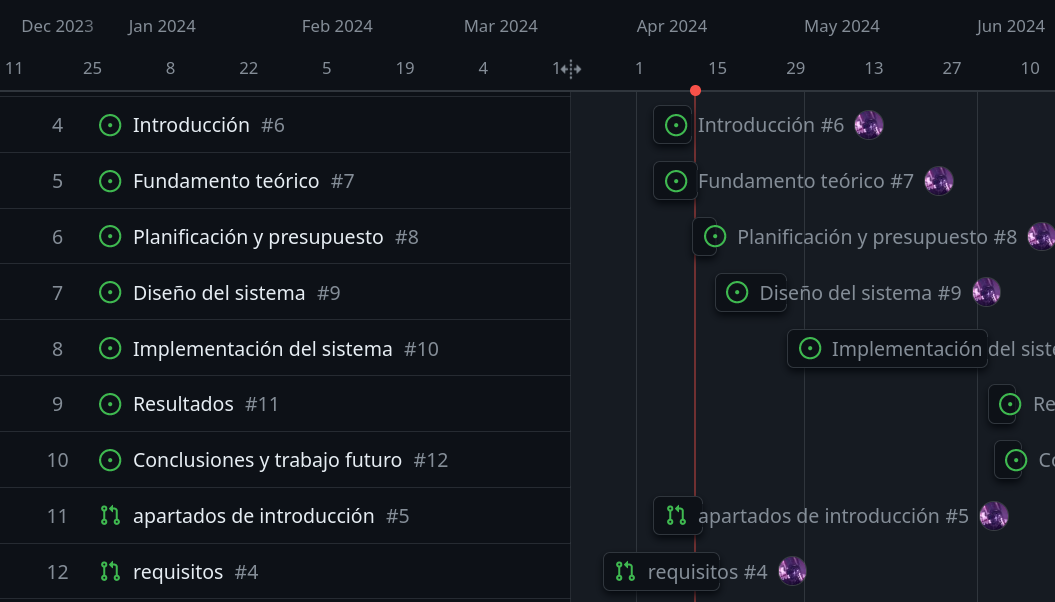
\includegraphics[width=0.9\textwidth]{roadmap.png}
			\captionof{figure}{Roadmap de apartados de la memoria}
		\end{minipage}
\end{itemize}


\subsection{Comunicación}\label{subsec:comunicación}
La comunicación con los tutores y con el equipo de desarrollo se considera fundamental para el
correcto desarrollo del proyecto. Puesto que el trabajo se desarrolla de manera presencial en
la oficina de la empresa, la comunicación con el equipo de desarrollo se realiza de manera
frecuente y directa, mientras que la comunicación con los tutores se realiza de manera remota
pero igual de frecuente, manteniendo el contacto mediante correo electrónico y Teams para
pedir revisiones e informar sobre el estado del trabajo en todo momento.

\subsection{Plataformas de planificación}\label{subsec:plataformas}
Con el objetivo de facilitar las tareas de desarrollo y cumplimentar los requisitos por parte
de la empresa, se utilizan las siguientes plataformas y herramientas de desarrollo para la
fabricación del proyecto:

\begin{itemize}
	\item \textbf{GitHub}: Plataforma de desarrollo colaborativo para el desarrollo del proyecto.
		Se utiliza para la gestión de tareas, seguimiento de desarrollo, documentación y
		colaboración.
	\item \textbf{Atlassian suite (\emph{Jira, Bitbucket})}: Suite de herramientas de gestión de proyectos
		y desarrollo colaborativo. Se utiliza para el desarrollo y documentación del proyecto de
		parte de la empresa.
	\item \textbf{Microsoft Teams}: Herramienta de comunicación y colaboración en tiempo real.
	\item \textbf{Microsoft Outlook}: Herramienta de comunicación por correo electrónico.
\end{itemize}

\newpage{}
\section{Planificación inicial}\label{sec:planif_inicial}
Como se ha mencionado anteriormente, se utiliza la metodología \textit{Scrum} para la planificación
y desarrollo del proyecto. En la figura \ref{fig:backlog} se puede ver el \textit{backlog}
de tareas que se planifican en el proyecto.

\begin{figure}[H]
	\centering
	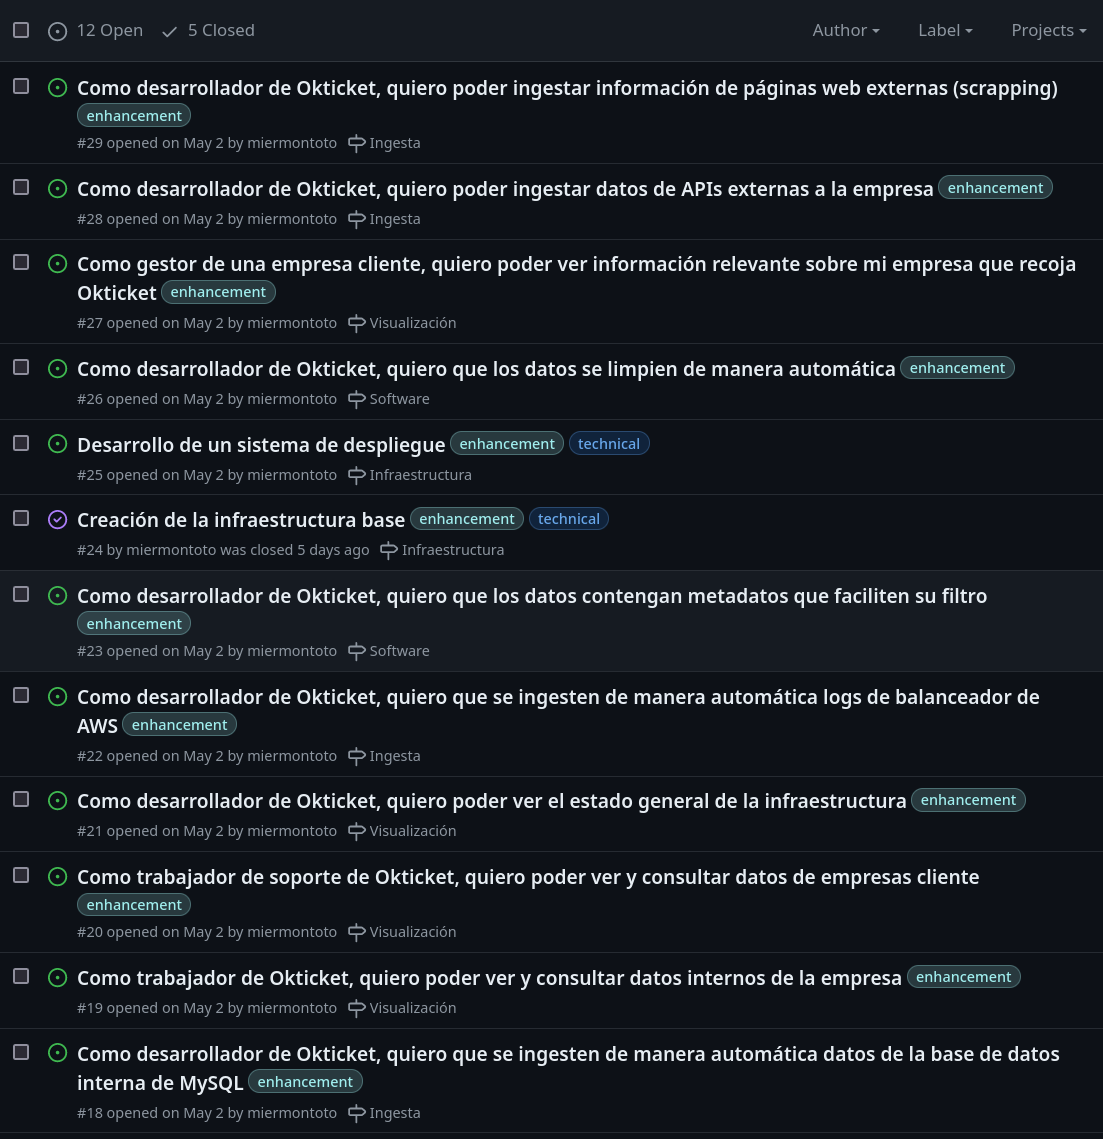
\includegraphics[width=\textwidth]{backlog.png}
	\caption{Planificación inicial del proyecto}
	\label{fig:backlog}
\end{figure}

Las tareas anteriores se clasifican y categorizan según su prioridad y tamaño, haciendo uso de la
estrategia de tallas de camiseta para esta última. En el tablero \textit{Kanban} (ver figura
\ref{fig:kanban}) se puede ver en todo momento el estado de las tareas, su progreso y sus
características. El listado de tareas iniciales (ordenado según su prioridad) es el siguiente:

\begin{table}[H]
	\centering
	\begin{tabular}{|p{0.7\linewidth}|c|c|}
		\hline
		\textbf{Tarea} & \textbf{Prioridad} & \textbf{Tamaño} \\
		\hline
		\hline
		Creación de la infraestructura base (técnica) & P0\cellcolor{red!50} & L\cellcolor{orange!50} \\
		\hline
		Como desarrollador de Okticket, quiero que la arquitectura se despliegue y orqueste de manera automática & P0\cellcolor{red!50} & XL\cellcolor{red!50} \\
		\hline
		Como desarrollador de Okticket, quiero que se ingesten de manera automática datos de la base de datos interna de MongoDB & P0\cellcolor{red!50} & M\cellcolor{yellow!50} \\
		\hline
		Como desarrollador de Okticket, quiero que se ingesten de manera automática datos de la base de datos interna de MySQL & P0\cellcolor{red!50} & M\cellcolor{yellow!50} \\
		\hline
		Como desarrollador de Okticket, quiero que los datos se limpien de manera automática & P0\cellcolor{red!50} & M\cellcolor{yellow!50} \\
		\hline
		Como trabajador de Okticket, quiero poder ver y consultar datos internos de la empresa & P1\cellcolor{orange!50} & L\cellcolor{orange!50} \\
		\hline
		Como desarrollador de Okticket, quiero que se ingesten de manera automática logs de balanceador de AWS & P1\cellcolor{orange!50} & S\cellcolor{green!25} \\
		\hline
		Como desarrollador de Okticket, quiero poder ver el estado general de la infraestructura & P1\cellcolor{orange!50} & L\cellcolor{orange!50} \\
		\hline
		Como desarrollador de Okticket, quiero que los datos contengan metadatos que faciliten su filtrado o búsqueda & P2\cellcolor{yellow!50} & S\cellcolor{green!25} \\
		\hline
		Como trabajador de Okticket, quiero poder ver y consultar datos de empresas cliente & P2\cellcolor{yellow!50} & M\cellcolor{yellow!50} \\
		\hline
		Como gestor de una empresa cliente, quiero poder ver información relevante sobre mi empresa que recoja Okticket & P2\cellcolor{yellow!50} & L\cellcolor{orange!50} \\
		\hline
		Como desarrollador de Okticket, quiero poder ingestar datos de APIs externas a la empresa & P2\cellcolor{yellow!50} & L\cellcolor{orange!50} \\
		\hline
		Como desarrollador de Okticket, quiero poder ingestar información de páginas web externas (\textit{scraping}) & P2\cellcolor{yellow!50} & XL\cellcolor{red!50} \\
		\hline
	\end{tabular}
	\caption{Listado de tareas iniciales}
	\label{tab:initial_tasks}
\end{table}

\newpage{}
\section{Presupuesto}\label{sec:presupuesto}
